\subsection{Kiểm thử các xử lý logic}

Để đảm bảo hệ thống hoạt động ổn định và chính xác, các xử lý logic của hệ thống cần được kiểm thử kỹ lưỡng. Các kiểm thử này sẽ giúp phát hiện và sửa chữa các lỗi trong mã nguồn, đảm bảo rằng các chức năng của hệ thống hoạt động như mong đợi. Các kiểm thử này bao gồm kiểm thử đơn vị (Unit Testing) và kiểm thử API (API Testing).
\subsubsection{Kiểm thử đơn vị}


\textbf{Phạm vi kiểm thử}

Phạm vi kiểm thử đơn vị cho ứng dụng Smart Gallery bao gồm kiểm thử các hàm xử lý và các lớp xử lý logic của 2 server labeling ảnh và server tạo video. 

\textbf{Môi trường kiểm thử}

Môi trường kiểm thử cho các xử lý logic gồm có: 
\begin{itemize}
    \item JestJS\cite{jestJS}: là một công cụ được sử
    dụng để kiểm thử đơn vị được tích hợp sẵn trong NodeJs.
    \item pytest\cite{pytest}: là một thư viện kiểm thử đơn vị mạnh mẽ và linh hoạt cho Python. Kết hợp song song với unittest\cite{unittest}, pytest giúp kiểm thử các hàm xử lý logic của server labeling ảnh.
\end{itemize}

\textbf{Kết quả kiểm thử}

Độ phủ và kết quả kiểm thử xử lý logic như Hình \ref{fig:jest-testing}, Hình \ref{fig:pytest-coverage} và Hình \ref{fig:pytest-testing}.

\begin{figure}[H]
    \centering  
    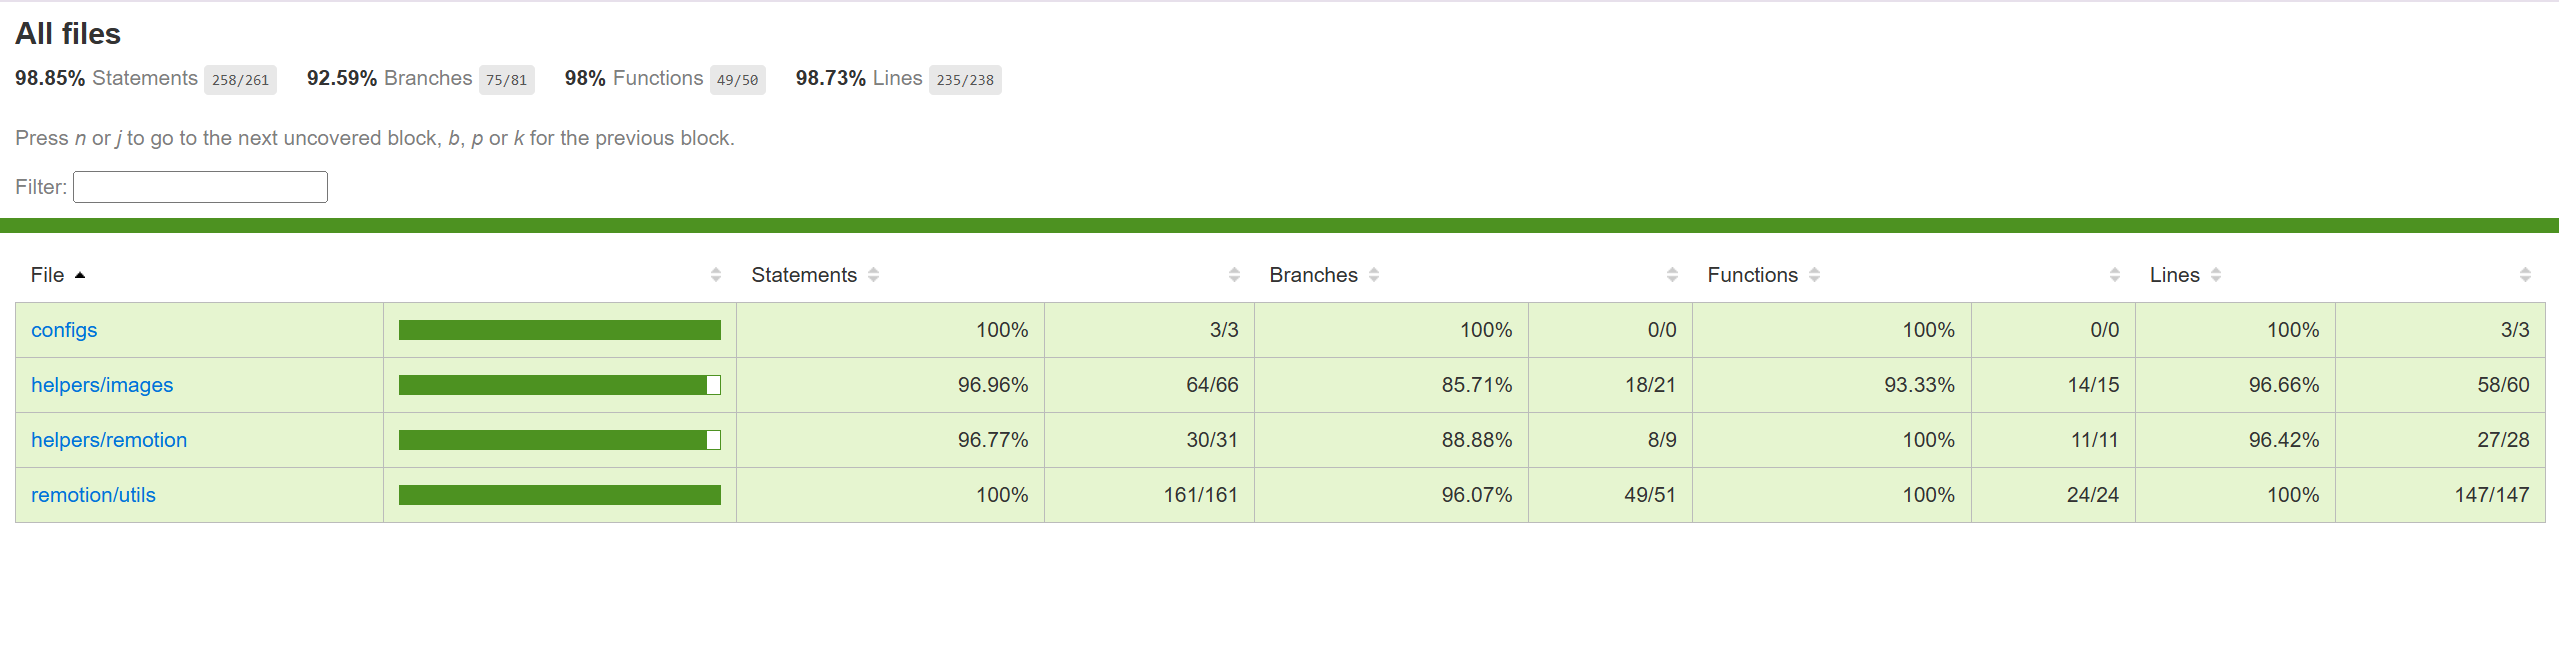
\includegraphics[width=1\textwidth]{figures/c4/4-3/jest.png}
    \caption{Độ phủ kiểm thử xử lý logic với JestJS.}
    \label{fig:jest-testing}
\end{figure}

\begin{figure}[H]
    \centering  
    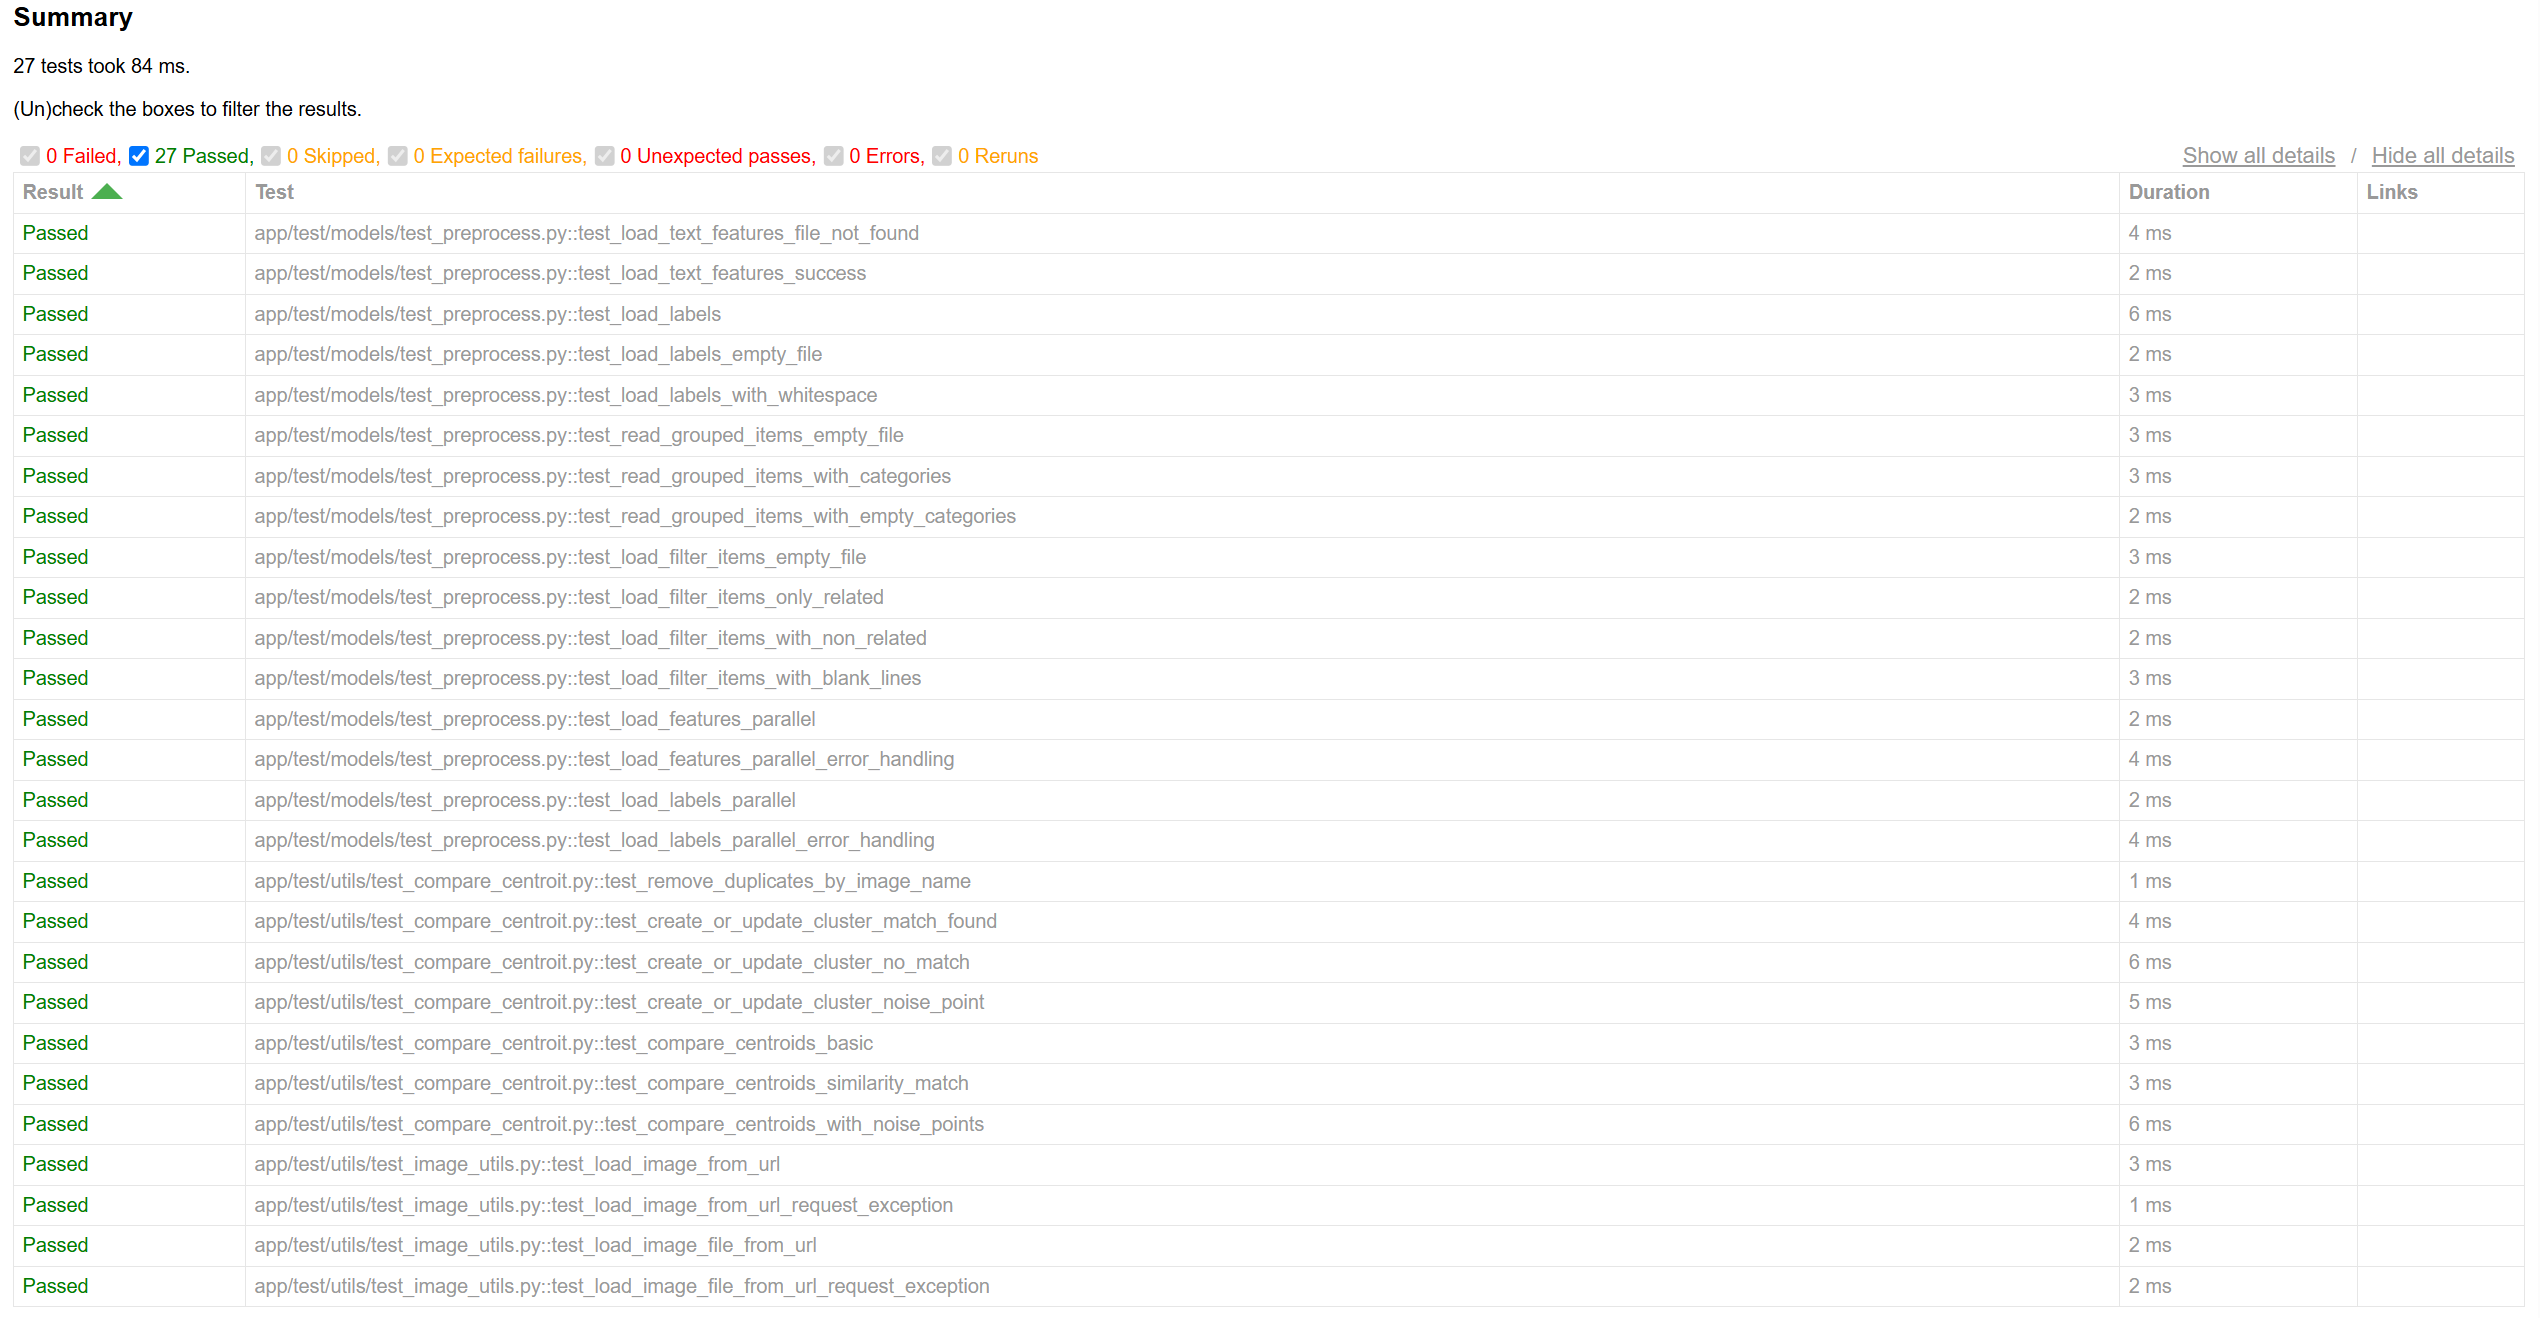
\includegraphics[width=1\textwidth]{figures/c4/4-3/pytest.png}
    \caption{Kết quả các ca kiểm thử đơn vị với Pytest.}
    \label{fig:pytest-coverage}
\end{figure}

\begin{figure}[H]
    \centering  
    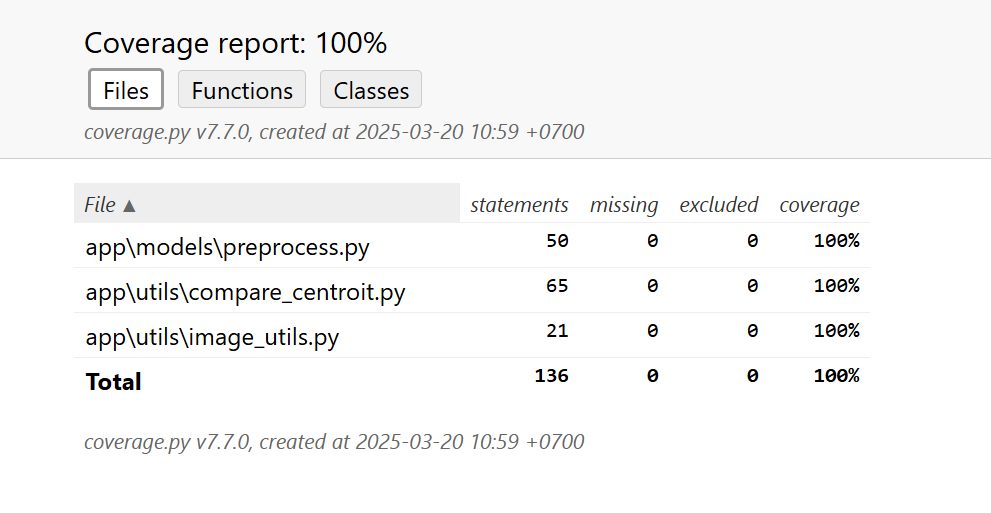
\includegraphics[width=1\textwidth]{figures/c4/4-3/pytest_2.png}
    \caption{Độ phủ kiểm thử xử lý logic với pytest.}
    \label{fig:pytest-testing}
\end{figure}


\subsubsection{Kiểm thử API}